\documentclass[a4paper,11pt,report]{report}
\usepackage[pdftex]{graphicx}
\usepackage{mathtools}
\usepackage[margin=1in]{geometry}
\usepackage{float}
\usepackage{lscape}
\usepackage{pdfpages}
\usepackage{epsfig}
\usepackage{epstopdf}
\DeclareGraphicsExtensions{.pdf,.png,.jpg,.eps}
\setlength{\parindent}{0in}
\begin{document}

\title{Slice of Pie}
\author{Andreas Precht Poulsen, Christian Rostrup Nielsen, Mark Thorhauge \& Mikkel Funch}
\date{17-12-2012}
\maketitle

\section{Introduction}
This report is written in November and December 2012 in a four-week project at the IT-University of Copenhagen under supervision of course responsible Jakob E. Bardram and Dario Pacino as well as Teachers assistants Mads Frost, Simon Terkildsen and Nicolai Skovvart. In the project a document management system was developed with a web interface and a stand-alone client. The system deals with problems such as synchronizing, sharing and merging of documents.

\tableofcontents
\listoffigures

\section{Vision}
\paragraph{Introduction}
We envision a document management system that makes it possible to work together on the same document both through a browser and a windows application. We imagine that the client is very similar to the web interface. The system must be flexible, allowing the user to manage documents both online and offline and merge changes. The system shall be equipped to deal with extensions and coupling of additional clients or persistence solutions. \\
\subsection{Positioning}
\paragraph{Problem Statement} 
We are required to develop a system which allows the user to manage documents through a web interface and share it with other users. Changes made to the same document shall be merged and documents can be downloaded for offline use to a stand-alone client. Documents can contain images and all revisions of a document is visible through a revision history.

\newpage

\section{Software Analysis}
	\subsection{Use cases}
	The product is defined from the requirements. The functional requirements are represented as use cases that the system should support. These are brief descriptions of the use cases.
	\begin{itemize}
	\item User wants to create a document. He or she specifies a title for the document and the document is displayed in the specified folder or project.
	\item User wants to edit a document. He or she has selected a document and the textual content is displayed. Changes can be saved or synchronized depending on whether the user uses the web interface or the client.
	\item User wants to delete a document. He or she has selected a document before and a blank document screen is shown after the operation.
	\item User wants to share a document with another user. The target user's account identification is specified and the server's status response is displayed.
	\item User wants to save a document offline. A document is selected and after the button is pressed, nothing changes in the view.
	\item User wants to sync his version with the server version. He or she has selected a document and if an eventual conflict is raised. The user solves the conflict and in both cases the final version is displayed.
	\item User wants to format his document. The user has completed edit document first and can mark text for different format types.
	\item User wants to insert a picture. He or she specifies the URL of the picture and the picture is shown in the document.
	\item User wants to  download his document for offline use. The user completes the sync use case.
	\item User wants to view his revision history. A document is selected and the list of document revisions are shown.
	\item User wants to rollback a change. The user completes the show revision history use case and selects the revision to rollback to. The document is shown as it was in the selected revision.
	\item User wants to organize document into project/folders. The user selects a document and a folder to put it in. The document is displayed in the folder.
	\item User wants to download his document to his local folder. He or she selects a document and it is downloaded via the browsers download framework.
	\end{itemize}
	\subsubsection{Fully dressed use cases}
\textbf{Name:} Manage document \\
\textbf{Scope:} Client and website \\
\textbf{Level:} User goal \\
\textbf{Stakeholders and Interests:}
\begin{itemize}
	\item User wants to create, read, edit or delete and be able to observe the outcome.
\end{itemize} 
\textbf{Preconditions:}
\begin{itemize}
	\item If user uses the website, he must be online.
\end{itemize} 
\textbf{Main success scenario:}
\begin{itemize}
	\item User creates or changes a document and is able to observe the resulting state of his repository.
\end{itemize} 
\textbf{Extensions:}
\begin{itemize}
	\item a. At any time system fails:
	\item Rollback any changes that was made while the system failed.
	\item Restart the system and change the state to before the failure was detected.
\end{itemize} 

\textbf{Name:} Synchronize document \\
\textbf{Scope:} Client and website \\
\textbf{Level:} User goal \\
\textbf{Stakeholders and Interests:}
\begin{itemize}
	\item User wants to sync his document and be notified about conflicts or fast-forward merge.
\end{itemize} 
\textbf{Preconditions:}
\begin{itemize}
	\item If user uses the website, he must be online.
	\item If user uses the client he or she shall be logged on.
\end{itemize} 
\textbf{Main success scenario:}
\begin{itemize}
	\item User syncs a document and has the opportunity to deal with conflicts and observe the resulting document and its state.
\end{itemize} 
\textbf{Extensions:}
\begin{itemize}
	\item a. At any time system fails:
	\item Rollback any changes that was made while the system failed.
	\item Restart the system and change the state to before the failure was detected.
\end{itemize} 

\newpage

	\subsection{Supplementary specification}
	The non-functional requirements are structured and defined with FURPS+. \\ \\
\textbf{Functionality} \\
The program shall support a minimum of functions.
\begin{itemize}
\item The functions include management(CRUD\footnote[6]{Abbreviation for Create, Read, Update and Delete}), sharing, organizing and local and online storage of documents.
\item Organization of documents includes creation, deletion and repositioning of folders.
\item For use cases to be completed online, the user shall be able to create a user.
\end{itemize}
\textbf{Usability} \\
The program shall be easy to use, mainly because of the limited features it shall support. Functions shall be intuitivly grouped and the number of windows required for each task shall be limited to two. Almost all features shall be visible in one window. Users used to using the web version shall have almost no introduction to be able to use the client efficiently.
\begin{itemize}
\item Anyone beyond the age of 13 shall be able to understand the program terminology.
\item No task may take more than 10 minutes(writing of document text subtracted) to complete for a new user of the system.
\item All features shall have minimal help documentation explaining how the feature is used, what it requires and what it returns.
\end{itemize}
\textbf{Reliability} \\
The program shall be reliable to an extent that does not compromise security or functionality. The server shall be able to handle crashes.
\begin{itemize}
\item The client shall be able to complete as many tasks as possible without connection to the server.
\item Failure shall maintain the content of the persistence storage as before the failure.
\end{itemize}
\textbf{Performance} \\
The program shall have reasonable performance. This means that no operation shall take longer than defined in the quality scenarios with a bandwidth with more than 2 mBit/s and a processor with a frequency equal to or greater than 1 GHz. However for extension of data compression and/or the merge algorithm response time can vary depending on the server processor and the size of the document involved in the operation.
\\ \\
\textbf{Supportability} \\
The program shall be very extensible and adaptable. This includes linking the server to additional clients, and third party software, and/or persistence solutions. The program architecture may not limit scalability in case the program shall handle an increasing amount of users.
\begin{itemize}
\item The system shall only be running on Windows OS\footnote[7]{Abbreviation for Operating System} supporting .NET 4.0 framework. This includes both client and server.
\item Linking of additional clients and/or third party software shall require a minimum of changes to the server and no change to the architecture.
\end{itemize}

	\subsection{Domain model}
	Domain model for our initial scope. Projects are omitted to simplify implementation.
	\begin{figure}[H]
  \centering
	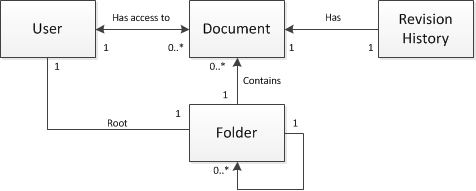
\includegraphics[]{./DomainModel}
\caption{Domain model }
\end{figure}
	\subsection{Technical analysis}
		\subsubsection{Analysis of persistent storage}
		A central part of the system is data storage because the majority of the use cases relies on retrieving or saving data online or offline. The client application requires data storage for a few users, making the performance for retrieving documents less relevant. The 			server stores data for all users of the system, which in a large system could reduce performance for most use cases. Therefore the performance of the system is improved by storing data in a database. Another thing to consider is the flexibility that a DBMS brings. If 		the system shall support additional use cases in the future, requiring new data retrieval queries, the DBMS can maintain sufficient performance with secondary indexes. \\ \\
		The content of the documents which should be stored in the database have very variable size. As databases shall allocate a certain amount of space for each attribute in each tuple, storing the content of the document in the database raises a problem. It is not 			intended to make any restrictions on the length of a document. To solve this the database could store the path to a file, which is located in the servers file system. The file system is very efficient at retrieving files at a specific location. However, this solution makes 			transaction rollbacks and data recovery more complicated and less reliable. The system does not need the transaction functionality of the DBMS, but recovery and backup could be important as users store valuable documents in the system. The performance gained 			by using this solution is not easy to predict. However, a research paper\cite{Russel} suggests that it is faster with objects over a certain size, which very large documents could obtain. If the database were to contain pictures, supporting it with a file system 			would improve performance.  \\ \\
		The relational database should contain the objects modeled in the Domain Model. Users and folders have two separate tables in the database. Documents can be modeled in two ways, because all editions of a document should be saved. The simplest one is to make a 		single table for all documents and editions of documents. An edited document is simply saved as a new document with a common key to link it to the previous version. As document has a title, and the edited document should have the same, this duplicates data and 			violates BCNF. The original document is identified only by comparing all the editions to find the earliest creation data. Clearly this simple solution has some drawbacks. \\ \\
		Another solution creates a second table with document revisions to distinct between original documents and revisions. This makes retrieving of the original document and retrieving of revisions(for revision history) simpler and faster. It does complicate the task of 			loading the latest document because a check for the eventual existence of a revision shall be done, alternatively the document with the latest time stamp is the latest revision too. \\ \\
		A considerable benefit with the document revision model and the filesystem support is the ability to save diff\footnote[1]{File containing the difference between two files as an edit script} files in the database. Diff files are smaller than document files and to maintain 			good performance, these should be stored in the database. This is a very effective data compression mechanism, which could be important if lots of revisions are made of large documents. This improvement would require the diff algorithm to work efficiently, 				else it would put a considerable CPU requirement on the server, depending on the time complexity of the algorithm and the number and frequency of synchronize requests.
		
		\subsubsection{Analysis of the merge problem}
		If a user of the system edits a document, which simultainasly has been modified by another user, a conflict can occur. Because both users can modify the same part of the document, no unambiguous solution to the conflict exists. However the system can help the 			users solve the conflict by highlighting the changed parts and make his choice of what to keep and what to delete easier. If the two have modified different sections of the document, a conflict can be avoided by doing a three-way merge. The problem is usually 			solved by a diff3 algorithm which uses the diff2 algorithm. Therefore the first problem to analyze is to find the minimal difference between two documents. \\ \\
		The problem is very similar to the longest common subsequence problem which finds the shortest set of insertions and deletions(editscript) that transforms one string into another string. In this case the system shall highlight only the lines that differs to the user. It is 			solved by the diff2 algorithm, which have a time complexity of \begin{math}O(ND)\end{math}\cite{Eugene}\footnote[2]{N being the sum of the length of the strings and D being the length of the edit script}. The algorithm is complex to implement. However it is easy 			to implement an algorithm with \begin{math}O(N^2)\end{math} and \begin{math} \Omega (N)\end{math} time complexity and no guarantee for returning the edit script, which is the shortest existing edit script. \\ \\
		The \begin{math}O(N^2)\end{math} algorithm is sufficient for most uses, but could be slow for large documents. Another thing to consider is the behavior of the diff3 algorithm if it is based on a \begin{math}O(N^2)\end{math} algorithm which does not guarantee      		to return the shortest edit script. This could cause the diff3 algorithm to have unpredictable behavior. \\ \\
		As mentioned in the analysis of the persistence storage, the diff2 algorithm has important data compression uses.

		\subsubsection{Analysis of UI technologies}
		The available UI technologies consists of ASP.NET paired with Windows Forms, and WPF\footnote[3]{Windows Presentation Foundation} supported by Silverlight for web presentation. The most significant difference between the two options is that all UI components in WPF is writen in XAML, which can be directly interpreted in Silverlight, while components made in Windows Forms can not be reused in the ASP.NET web presentation. This results in twice as much work for adding components to both interfaces, compared to WPF with Silverlight. WPF and Silverlight is technologies that we have never used before, and therefore it costs alot of resources to use this technology, aswell as adding an element of risk to the project. However for further extension of the system, WPF is very advantageous as only half the effort is put into implementing additional graphical components. As for framework support, WPF is the leading technology, making it a better choice for future compatibility. It also offers high level components such as Rich Text Box\footnote[4]{Component for formating and illustrating other components} which could prove important for further extension of the system and covering of less prioritized use cases.

\section{Architectural analysis}
\subsection{Architectural factors}
In this section the architectural requirements for the system is analyzed based on the non-functional requirements. The most important architectural factors are identified to make the architectural decisions.
\subsubsection{Evolution points}
The architecture shall support these evolution points.
\begin{itemize}
\item Server storage of additional large binary objects such as pictures.
\item Communication with additional client types.
\item Communication with third party software.
\item Replication of persistence storage.
\item Implementation of new UI elements
\item Communication with multiple clients.
\end{itemize}
\subsection{Architectural decisions}
\subsubsection{Reliability and Fault Tolerance}
The fail strategy for the server is to restart completely and be running within 2 minutes. If the technical services fail, such as web connection, database or file system no alternative is required resulting in the entire server failing. Client is separated from the server, which means that only the use cases that require server connection fails on server failure. This does not have any significant effect on the architecture.
\subsubsection{Supportability}
The architecture shall support implementation of additional persistence solutions to replicate and/or store existing and/or new object types. To achieve this we want all persistence solutions to be joined in a fascade. This limits the impact that implementation of new functionality and change of existing functionality will have on the rest on the system. It also simplifies the API of the persistence storage subsystem as well as allows large binary files to be stored in the file system as discussed in the technical analysis. This encapsulation of the subsystem allows some of the evolution points to be implemented with minimal complications. \\ \\
The architecture shall allow an arbitrary number of clients to connect to the server and support different connections types without making avoidable changes to the server. This is achieved by using a Web Service entry  point to the server. This solution simplifies the development. Communication with third party software is easier with web services, because the entry point of the server is equal for all communication.\\ \\
To allow easy implementation of new UI elements, the web interface and the client shall be based on the same UI framework. The code representation of the components shall be identical resulting in parallel development of the client and the web interface. New UI components shall only be written once to be implemented in both the web interface and the client interface. \\ \\
The architecture shall be designed with general software quality factors such as low coupling and cohesion in mind. This involves designing the client with the MVC\footnote[9]{Abbreviation for Model View Controller} structure. 
\subsubsection{Performance}
The non-functional requirements for performance is not very restrictive and this requirement will not influence the architecture. Any performance drawbacks the Web Service solution might bring is outside the scope of this analysis.


\section{Software Design}
\subsection{Server class diagram}
\begin{figure}[H]
  \centering
\includegraphics[]{./classdiagramserver1}
\caption{Class diagram modeling the server without PersistentStorage}
\end{figure}

\begin{figure}[H]
  \centering
\includegraphics[]{./classdiagramserver2}
\caption{Class diagram modeling the PersistentStorage component}
\end{figure}

\subsection{Client class diagram}
\begin{figure}[H]
  \centering
\includegraphics[]{./classdiagramclient}
\caption{Class diagram modeling the client}
\end{figure}

\subsection{Interaction diagrams}
Interaction diagrams are included in Appendix B.

\subsection{Description of classes and responsibilities}
The most important classes are described and their responsibilities and collaborators are briefly explained.
\paragraph{Server Controller}
The server controller handles all communication across all components. The Service component calls the controller. The Controller calls the PersistentStorage to save objects and the model to resolve merge conflicts.
\paragraph{PersistentStorage}
The PersistentStorage handles persistent storage of objects. It calls FileSystemHandler and DAO to store respectively document content and other objects on the server.
\paragraph{Model}
The Model handles merging of documents. The Controller uses it to resolve merge conflicts and return edit scripts.
\paragraph{Service}
The Service handles all online requests. It calls the Controller. Uses service classes to marshall and unmarshall objects.
\paragraph{Client Controller}
The Controller is responsible for handeling communication with the server's Service and call PersistentStorage(Local), Security and Session as well as the MainWindow.
\paragraph{MainWindow}
Contains all GUI components represented by XAML code. It calls the Controller's methods and contains the events.
\paragraph{Session}
Session stores information about the user and the document in focus. It is called by the Controller.
\paragraph{Security}
The Security class encrypts passwords with the SHA1 algorithm used by the System.Security.Cryptography package.

\subsection{Use of design patterns}
\subsubsection{Component Design Patterns}
\paragraph{Singleton}
Singleton design pattern is used to ensure that only one instance of a class is instantiated and used. We have used singleton in Controllers, Models, PersistentStorage, FileSystemHandler and DAO\footnote[8]{Abbreviation for Data Access Object}. All implementations include lazy instantiation, which does not have any noticeable impact, as the classes does not contain fields other than the instance.
\paragraph {Composite}
The composite design pattern is used in the relationship between folders. In the database, all folders have a parent id, which is a reference to the containing folder. This is the way folders are modeled in common operating systems and because we want to replicate the database data in the client's file system, this design has been adopted.
\paragraph {Facade}
The PersistentStorage class is a facade that joins the functionality of the file system with the functionality of the database. The reason for adopting this design is to allow further extension of the data storage component. Alternatively all functionality would be in the DAO, which would complicate understanding of the system and separation of functionality for eventual switching of components. If eventual replication of the data in PersistenceStorage were to be implemented, this design would simplify the task.
\paragraph {Database Mapper Pattern}
Although not implemented by us, the automated code generated by ADO.NET entity framework uses the Database Mapper Pattern to generate objects from the database and store objects to database tables.

\section{Architectural Design}
\subsection{Architectural Patterns}
\subsubsection{Model View Controller}
The server is roughly structured using the MVC design pattern. The server has a middle link, the webservice, between the web UI and the controller. The client has a controller which separates the UI and the model(Session and PersistentStorage), hence it follows the principle strictly. The pattern is used to easily replace components, lower coupling and increase cohesion.
\subsubsection{Client-Server}
The communication between the client and the server follows the client server design pattern. An alternative design pattern is peer-to-peer, which would complicate the implementation greatly. For all clients to be able to work independent of each other, the client server design pattern is adopted.
\subsubsection{Quality scenarios }
All quality scenario response time limits are with the bandwidth and processor specified in the supplementary specification under performance. Normal server load is defined as 50 users using the server with an average of 5 requests per minute and a standard deviation of 0,7.
\paragraph{Share document}
When a user wants to share a document he or she gets response from the server within half a seconds in 95\% of the cases under normal server load.
\paragraph{Create document} When a user synchronizes a document an eventual merge conflict is returned within 1,2 seconds in 95\% of the cases under normal server load.
\paragraph{Save document offline} When a user saves a document offline on the client the document content is in the file system within one tenth of a second in 98\% of the cases.
\paragraph{Create folder} When a user creates a folder it is visible to the user and reflected in the database within 0,4 seconds in 95\% of the cases under normal server load.

\subsection{Factor tables}
Factor tables are included in Appendix B.
- 
\subsection{Architectural Views}
The relevant architectural views for this system are the Logical view, the physical view and the use case view.
\newpage
\subsubsection{Logical View}
The logical view consists of the package diagram below.
\begin{figure}[H]
  \centering
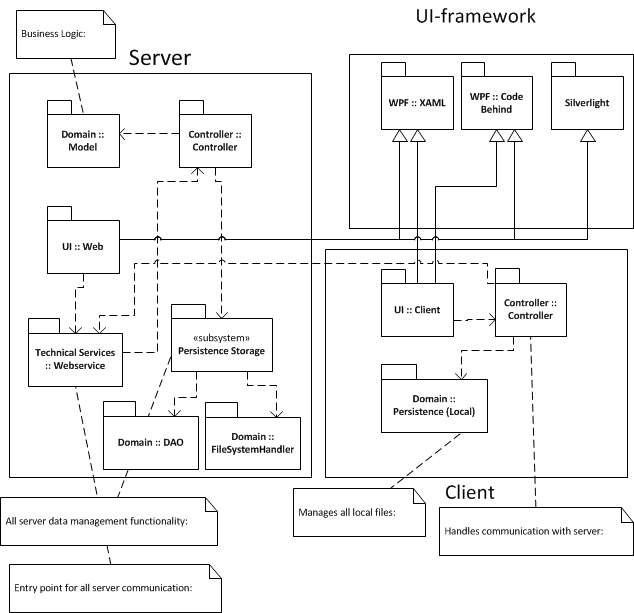
\includegraphics[]{./logicalview}
\caption{Package diagram}
\end{figure}
\newpage
\subsubsection{Physical View}
The physical view consists of the deployment diagram below.
\begin{figure}[H]
  \centering
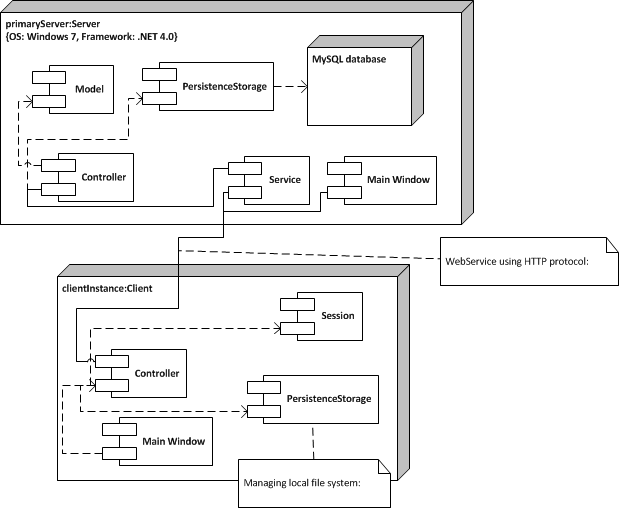
\includegraphics[]{./deploymentview}
\caption{Deployment diagram}
\end{figure}
\newpage
\subsubsection{Use Case View}
The use case view consists of a use case model, operation contracts, system sequence diagrams\footnote[10]{Included in Appendix B} and use case text\footnote[11]{Included in Software Analysis}.
\begin{figure}[H]
  \centering
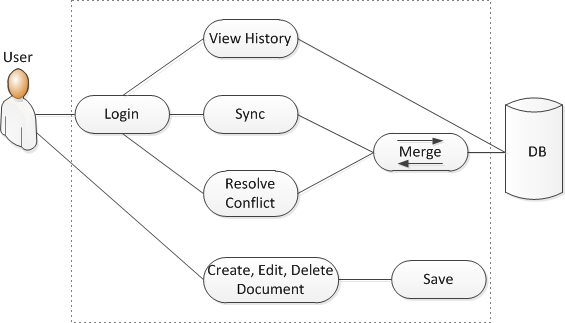
\includegraphics[]{./UseCaseDiagram}
\caption{Use case diagram}
\end{figure}
\paragraph{Operation Contracts}  \mbox{} \\
Operation contracts can be found in Appendix A.

\section{Testing}
\subsection{Testing Objective}
The objective of tests is to discover eventual failures or bugs in internal components by unit testing and in the entire system by integration and system testing. The focus is to make the core functionality of the system reliable, however eventual failures or performance decrease evoked by overloading the webservice or persistence storage with request or data is not our focus. The level of testing that most resources have been invested in is unit testing, as the internal workings of the system is subject to the highest risk factors and changes. As a SCRUM development process encourages lots of changes, automated tests help reducing the resources spent on reliability. 
\subsection{Unit testing}
All unit tests are in the TestProject. \\ \\
The DAO component of the persistent storage have been subject to unit tests. All methods are tested on an empty database to remove data duplication problems. As a drawback, this simplification removes eventual problems that arises when data exists in the database from the testing scope. Lots of the test methods have each other as dependency, making these unit tests effective at discovering failures, but not tracking them. This is as intended because such failures can be caused by different subsystems and dependencies. All the tests for DAO is contained in the DAOTest class. \\ \\
The mergeDocument method in the Model class has been subject to extensive unit testing. The method has important functionality and lots of different code paths. The unit tests cover all code paths and further whitebox testing and optimization has been easier with these. All the tests for mergeDocument is contained in the ModelTest class.
\subsubsection{Whitebox testing}
The mergeDocument method in the server Model class have been whitebox tested. All code paths have been examined in a debug view and as a result some of the conditional statements have been rewritten, because it had excessive checks. Even though it passed unit tests, an error existed, which the white box test revealed. As this method potentially is the most complicated and expensive method running on the server, it is the most relevant target for a whitebox test.
\subsection{System and Integration testing}
The Persistent Storage component of the server has been subject to integration testing. The storage component joins and encapsulates the functionality of the DAO and the FileSystemHandler, which together is responsible for all online data management. All functionality which involves both components(all operations involving documents) have been run and the desired result have been confirmed manually. The entire system have been tested by completing all the use cases and observing the desired result, both outside and inside the system. No additional effort has been put into pushing the system to borderline cases.
\subsection{Testing results}
The tests have proved some of the subsystems to be very reliable and secure, primary through unit tests. However the rest of the system could be more thoroughly tested, specifically with dozens of users sharing the same document while making asynchronous sync requests. The lack of such tests makes it impossible to prove or disprove the quality scenarios. \\ \\
The tests showed bugs listed below.
\begin{itemize}
\item When synchronizing all documents to the client for offline work and no editions have been made by the user, a document revision is made. When other users watches the revision history, they will observe an erroneous change to the document.
\item When the user tries to share a document before it is synchronized to the server the client crashes. This is due to the servers lack of knowledge of the document and the lack of handling of this exception.
\end{itemize}

\newpage
\section{Scrum}
	\subsection{Definition of done}
	Our DOD is defined by the following bullets:	
	\begin{itemize}	
				\item	Implement code
				\\ 	All code needs to be implemented in a functional manner.
				\item	Document code
					\begin{itemize}	
						\item Method summary + return parameters
						\\ All methods should be thoroughly documented to ease the understanding of their functionality. If a method is particularly complex it should furthermore be documented within the code to ease the understanding of the method steps.
						\item Properties and fields
						\\ Properties, along with regular fields, should be well documented and their names should indicate what they are used for.
					\end{itemize}
				\item	Testing
				\\ The program will be blackbox tested via unit tests to ensure the given methods are properly functioning.
				\item	Confirmation of artifacts
				\\ All textual artifacts should be read through and confirmed by at least one other person than the author
					\\ \\	
	\end{itemize}
	\subsection{Initial Product Backlog}
		The systems Product Backlog as delivered by the Product Owner.
  \begin{center}

		\begin{table}[H]
		\caption{Product Backlog for Slice Of Pie}
		\begin{tabular}{l c c}
		\hline \hline
		Item & Time estimate & Priority
		\\ \hline
		\\ User want to create a document & 3 & 1
		\\ User want to edit a document & 2 & 1
		\\ User want to delete a document & 3 & 2
		\\ User want to share a document with another user & 8 & 1
		\\ User want to save a document offline & 1 & 2
		\\ User want to sync his version with the server version & 20 & 1
		\\ User want to format his document & 2 & 5
		\\ User want to insert picture & 13 & 2
		\\ User want to download his docs to offline repos via the client & 13 & 2
		\\ User want to rollback a change & 0 & 3
		\\ User want to view his revision history & 2 & 4
		\\ User want to organize documents in projects/folders & 8 & 2
		\\ User want to download doc to his download folder without the offline client & 2 & 5
		\\ Create a database & 40 & 1
		\\ Create UI & 100 & 1
		\\ Create client/server & 40 & 1
  	 	\end{tabular}
		\end{table}
  \end{center}
	\subsection{Sprints}
		\subsubsection{Sprint 1}
			\paragraph{Sprint Planning Meeting}
			At the first Sprint Planning Meeting we choose the items we felt was of most importance in order to live up to the program expectations along with enabling the team to get a good start at the project.

			\paragraph{Sprint Backlog}
			The sprint backlog is included in Appendix B.
			\paragraph{Burndown Chart}
				\mbox{}\\
				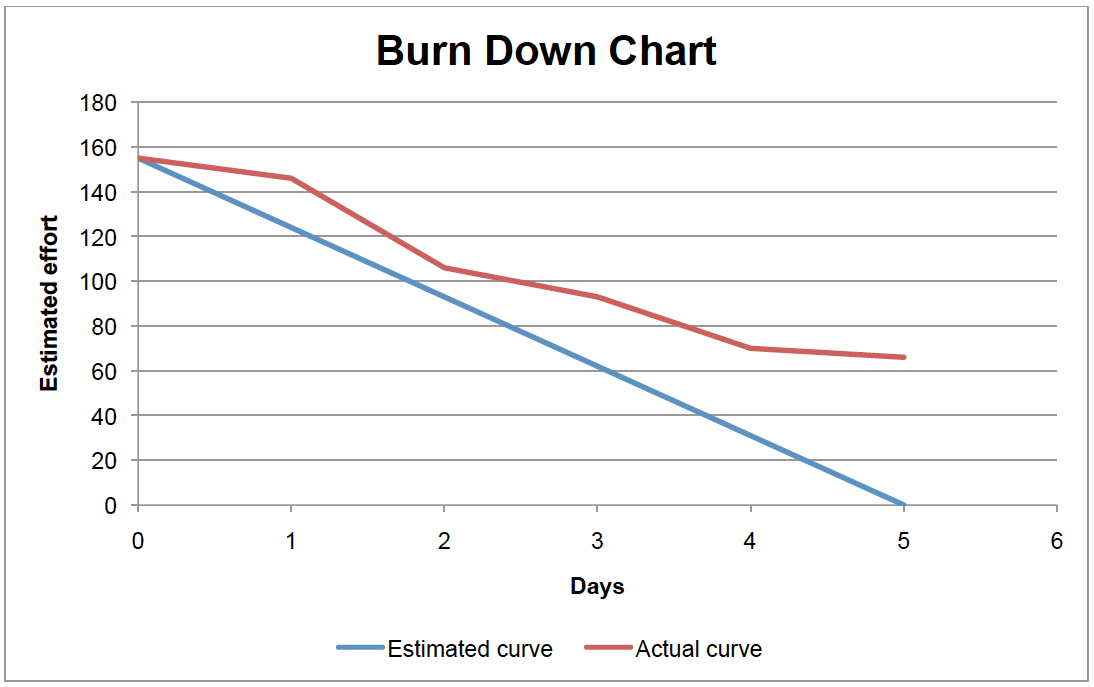
\includegraphics[width=12cm]{./Sprint1BurnDownChart.png}
			\paragraph{Daily Scrums}
		Each day we heared each other out, clearifying which sprint backlog items we completed and which we would begin with the day. In this way all members knew how the project was going and which items was being finished.
			\paragraph{Sprint Review}
			\paragraph{Sprint Retrospective}
				\subparagraph{Internal}
				Participants: Team and Scrum Master
				\\ 
				Looking back on our first Sprint of this particular project, it is easy to see some places where we can create more value in the following Sprints. What we need to stop doing, is using too much time arguing about the items for the Sprint Backlog. It seems more effective to chose the items (which has already been labeled with estimates and risks) and then start working on these from an early stage in the Sprint. From the Sprints Burn Down Chart we can tell, that we need to start on having a greater overview of the Items in the Sprint Backlog. By ensuring this, it will enable us to have a much more precise estimate of how far we have come with the chosen items, and it is also easier to add or remove items according to the time frame. What we need to continue doing, is having fun when we are working, whether being analysing, coding, writing, etc. It keeps up the good spirit and makes it easier to focus on the current task while still having the end goal ind mind.
				\subparagraph{External}
				Participants: Team, Scrum Master, Product Owner
				\\
The product that has been developed so far, is pretty decent compared to the number of items in the Sprint Backlog. We have some minor things within a few items that needs to be pushed forward into the next Sprint. Some of the �setbacks� has been because of unforseen obstacles that needed to be sorted out before it was possible to continue. When these are now cleared and the current issues has been resolved, it seems as though we are more than prepared for the next Sprint.
			\paragraph{Updated Product Backlog}
		\subsubsection{Sprint 2}
			\paragraph{Sprint Planning Meeting}
			At the beginning of spring 2 we choose the items that we needed to deploy the product. We needed to prioritize which use cases we felt most important for the program to succed.
			\paragraph{Sprint Backlog}
			The sprint backlog is included in Appendix A.
			\subsubsection{Burndown Chart}
\includegraphics[width=12cm]{./BurnDownChart.png}
			\paragraph{Sprint Review}
			\paragraph{Sprint Retrospective}
				\subparagraph{Internal}
				As we deploy the product after this sprint we feel that the retrospective serves a less important purpose than the last. We feel that the last retrospective helped us in optimizing the work. All group members where clear about the sprint items and that helped us coordinate our work.
				\subparagraph{External}
				We have completed almost all sprint backlog items and the product is almost ready for deployment. A few obstacles has made some of the testing and definition of done to be less thorough.

\newpage
\section{Conclusion}
In the project a large number of functional and non-functional requirements have been defined for the system, as well as lots of measures to evaluate it. Not all use cases have been covered, but the most crucial cases for the success of the system have been covered and works according to tests. The use cases has not been evaluated thoroughly by quality scenarios, making the performance requirements unverified. However our initial impression is that the performance is sufficient. The extendibility requirements are hard to verify with the resources given in this project. They are primarily based on the architecture, which have been implemented as analyzed in the architectural analysis. Overall we assess that the program comply with the non-functional requirements. \\ \\
We feel that the project could have been a lot better with an additional sprint, because it would allow more fundamental changes in the second sprint. Changes such as document metadata and local document metadata would have made the logic more clear and the code more readable, as well as testing easier. We would like to implement functionality to support additional use cases, which our design decisions are greatly influenced by.



\begin{thebibliography}{99}
\bibitem{Eugene}
  Eugene W. Myers,
  \emph{An O(ND) Difference Algorithm and Its Variations}.
  Department of Computer Science, University of Arizona, Tucson, AZ 85721, U.S.A

\bibitem{Russel}
  Russell Sears, Catharine van Ingen, Jim Gray
  \emph{To BLOB or Not To BLOB: 
Large Object Storage in a Database or a Filesystem}.
  Microsoft Research and University of California at Berkeley
  April 2006

\end{thebibliography}

\appendix

\chapter{Textual Artifacts}

\section{User manual}
The system can be used through a program and a website. The website is accessed through a browser and the client is downloaded through the website.
\subsection{Website}
You can create a user by clicking the Register button in the top left and type an email and a password. \\
All features the website offers requires a user.
\subsubsection {How to log in}
In the upper menu pane select Log In and enter user credentials. 
\subsubsection {How to create a document}
Just above the tree view click the create document button and specify a title in the pop up dialog.
\subsubsection{How to view an existing document}
Navigate through the document tree view on the left and click the document.
\subsubsection {How to edit a document}
Navigate through the document tree view on the left and edit the content in the middle. To save the changes click the Sync button. An eventual conflict can be resolved by editing the right document content and clicking the save merge button. The left document content is the version that was last synchronized.
\subsubsection {How to delete a document}
Navigate through the document tree view on the left and select the document. Click the delete button above the tree view.
\subsubsection {How to create a folder}
Navigate through the document tree view on the left and select the folder to contain the new folder. If no folder is selected it will be created in the root folder.
\subsubsection {How to move a document}
Navigate through the document tree view on the left and select the document, then click the move folder just above the tree view and specify the folder to contain the document. 
\subsubsection {How to view the history of changes to a document}
Navigate through the document tree view on the left and select the document, then click the History button.
\subsubsection {How to share a document with another user}
Navigate through the document tree view on the left and select the document, then click the share document button. Enter the email of the user.
\subsubsection {How to insert an image in a document}
Navigate through the document tree view on the left and select the document. Press the button with a landscape icon and type the URL to the image.
\subsection{Client}
The client offers functionality to create, edit and save documents offline. The functionality that requires internet connection is disabled when not logged in.
\subsubsection {How to log in}
Select File -> Log In, then enter user credentials.
\subsubsection {How to move a document}
Navigate through the document tree view on the left and select the document, then select Move document just above and specify the folder to contain the document. 
\subsubsection {How to save a document offline}
Click the Save document button in the right upper pane. Changes can be synchronized with the Sync button. 
\subsubsection {How to download all documents and editions of documents}
Click the Sync all button above the tree view. Non-conflicting saves made while offline will be synchronized to the server. 
\\ \\
See the website user manual for instructions on how to use the rest of the features.


\section{Technical Memos}
\subsubsection{2012-11-27 UI:}
When we had to choose the UI framework, we had two contestants which is Winforms and XAML. We chose XAML due to several reasons. Firstly it seemed more dynamic and easier to make a web-interface and a standalone client from roughly the same code. Secondly XAML seemed to fit our vision about making our program easy to maintain, since XAML is more dynamic and newer.

\subsubsection{2012-11-29 Images:}
When it comes to downloading the images in the document, we talked about two possible ways of doing it.
One was to store all the URL's in a database table, with a reference to the document. When downloading all documents, one would go through the database table and find all URL's with reference to one of the downloaded documents.
The other is to store the URL's in the document, and then loop through every document finding every URL.
Either way, we would download the images and store them in a local folder.

 We've chosen to keep the URL's in the document.

\subsubsection{2012-11-30 Database design}
We decided to let folder be an object restricted to a single user, which means that one document can be stored differently for each user sharing the document.
This makes deletion and syncing of documents easier to handle. It also limites the conflicts that can happen around folder names.
The table which handles the many-to-many relationship between user and document also stores the folder location.

\subsubsection{2012-12-05 Document revision server format}
We decided to make the server identify the document revision by name+"revision"+timestamp in the user's folder.
This will be a part of the path of the documentRevision path attribute in the database. The alternative would be fetching the id from the database
after creation and make it a part of the name. This is less efficient and requires both a write and a read.

\section{Operation Contracts}
\subparagraph{OC 1} \mbox{} \\
Operation: createUser(userMail:Mail, password: Hashed value of password) \\
\textbf{Exceptions}
\begin{itemize}
	\item If the given mail address is already in use the user will get an error and will have to start over.
	\end{itemize} 
\textbf{Preconditions}
\begin{itemize}
\item The user is online and has connection to the server
\item The user must type in the required information
\item The typed in mail address must not be in use already
\end{itemize} 
\textbf{Postconditions}
\begin{itemize}
\item Information about the user has been stored in the Database
\item The UI changed to a view in where the user is logged in
\end{itemize} 

\subparagraph{OC 2} \mbox{} \\
Operation: createDocumentOnline(docName:String, userId:int) \\
\textbf{Preconditions}
\begin{itemize}
\item The user is online and has connection to the server
\item The user is logged in
\end{itemize} 
\textbf{Postconditions}
\begin{itemize}
\item Information about the user has been stored in the Database
\item The UI changed to a view in where the user is logged in
\end{itemize} 

\subparagraph{OC 3} \mbox{} \\
Operation: createDocumentOffline(docName:String, userId:int) \\
\textbf{Preconditions}
\begin{itemize}
\item The user has installed the offline client which includes the offline repository
\end{itemize} 
\textbf{Postconditions}
\begin{itemize}
\item Information about the document was stored in the users local repository
\item The UI changed to the created document
\end{itemize} 

\subparagraph{OC 4} \mbox{} \\
Operation: editDocumentOnline(docId:int, userId:int) \\
\textbf{Preconditions}
\begin{itemize}
\item The user is online and has connection to the server
\item The user is logged in to the system
\item The user has access to the specified document
\end{itemize} 
\textbf{Postconditions}
\begin{itemize}
\item The user has access to the specified document
\item The UI changed to the specified document
\end{itemize} 

\subparagraph{OC 5} \mbox{} \\
Operation: editDocumentOffline(docId:int) \\
\textbf{Preconditions}
\begin{itemize}
\item The user has installed the offline client which includes the offline repository
\item The user has a saved document in his local respository
\end{itemize} 
\textbf{Postconditions}
\begin{itemize}
\item The document was changed
\end{itemize} 

\subparagraph{OC 6} \mbox{} \\
Operation: deleteDocumentOnline(docId:int) \\
\textbf{Preconditions}
\begin{itemize}
\item The user is online and has connection to the server
\item The user is logged in to the system
\end{itemize} 
\textbf{Postconditions}
\begin{itemize}
\item Information was changed in the database
\end{itemize} 

\subparagraph{OC 7} \mbox{} \\
Operation: deleteDocumentOffline(docId:int) \\
\textbf{Preconditions}
\begin{itemize}
\item The user has installed the offline client which includes the offline repository
\item The user has a saved document in his local respository
\end{itemize} 
\textbf{Postconditions}
\begin{itemize}
\item Information about the document was stored in the users local repository
\end{itemize} 

\subparagraph{OC 8} \mbox{} \\
Operation: syncDocument(docId:int) \\
\textbf{Preconditions}
\begin{itemize}
\item The user is online and has connection to the server
\item The user is logged in to the system
\end{itemize} 
\textbf{Postconditions}
\begin{itemize}
\item 1a: The server merged the document without any conflicts
\item 1b: The user got the option to solve a possible conflict
\end{itemize} 

\chapter{Diagrams}
\section{System sequence diagrams}
\begin{figure}[H]
  \centering
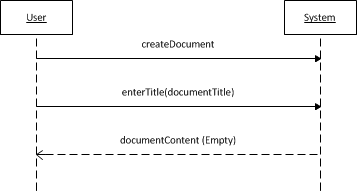
\includegraphics[]{./createdocumentssd}
\caption{System sequence diagram of Create Document}
\end{figure}
\begin{figure}[H]
  \centering
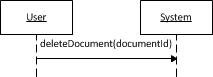
\includegraphics[]{./deleteDocument}
\caption{System sequence diagram of Delete Document}
\end{figure}
\begin{figure}[H]
  \centering
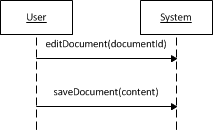
\includegraphics[]{./editdocumentssd}
\caption{System sequence diagram of Edit Document}
\end{figure}
\begin{figure}[H]
  \centering
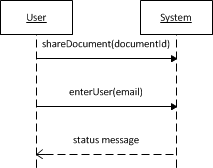
\includegraphics[]{./sharedocument}
\caption{System sequence diagram of Share Document}
\end{figure}
\begin{figure}[H]
  \centering
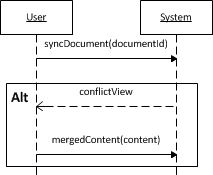
\includegraphics[]{./syncDocument}
\caption{System sequence diagram of Synchronize Document}
\end{figure}
\section{Factor tables}
\newpage
\begin{landscape}
\begin{table}
\small
\begin{center}
    \begin{tabular}{| p{3.3cm} | p{3.3cm} | p{3.3cm} | p{3.3cm} | p{3.3cm} | p{3.3cm} |}
    \hline
    Factor & Measures and quality scenarios & Variability (current flexibility and future evolution) & Impact of factor (and its variability) on stakeholders, architecture and other factors &  Priority for Success & Difficulty or risk\\ \hline
    \multicolumn{6}{|l|}{Reliability}
    \\ \hline
    Recovery from lost connection to server & If connection to server is lost, reconnection should be possible within the time frame of 2 minutes & The current version is supportive of upholding the most basic functionality in case the server connection fails. In 1.5 year, an online replication of the server (if one fails the other will take over) will have been made & The online replication has a high impact on stakeholders because they want reliable access to potentially important files. The replication also has a high impact on the server architecture because the webservice will have to be separated from the given servers & M & H
    \\ \hline
    Client failure & In case the client fails, all changes shall be temporarily saved in order for the user to choose which changes to save and which to discard & The current program does not support any of these functions. In 6 months this feature will be implemented into the program & It has medium impact on stakeholders since we do not have that many functions on the client side that can fail. It has low impact on the architecture since the required functions are relatively easy to implement into the current system & H & L
    \\ \hline
    Persistence storage internal failure & If the process of saving a file to the file system fails, no data should be saved in the DB to protect from inconsistent data. Likewise, if a save to the DB fails all coherent saves in the file system shall be rolled back & In the current system the functionality is already supported regarding failure in the file system. In one month, all operations regarding DB failure where the file system is involved will be supported & It will have a medium impact on stakeholders, since it would be somewhat irritating for a user to have a reference to a document that did not existed. It will have a low impact on system architecture & H & M
    \\ \hline
        \end{tabular}
\end{center}
\end{table}
\newpage
\begin{table}
\small
\begin{center}
    \begin{tabular}{| p{3.3cm} | p{3.3cm} | p{3.3cm} | p{3.3cm} | p{3.3cm} | p{3.3cm} |}
    \hline
    Factor & Measures and quality scenarios & Variability (current flexibility and future evolution) & Impact of factor (and its variability) on stakeholders, architecture and other factors &  Priority for Success & Difficulty or risk\\ \hline
 \multicolumn{6}{|l|}{Supportability}
        \\ \hline
        Support of large files, e.g. pictures, in server storage & Users shall be able to save large files in docs directly on server without support from external services & This functionality is currently supported by the persistence storage. An issue can be the space available for the file system compared to the number of users and their demands. All future concerns about this factor revolves around deployment and storage constraints & Low impact on stakeholders since there is no current support for the offline part either way. Also low impact on the the system architecture because persistence storage has been partitioned to avoid BLOB in the DB. & M & L
        \\ \hline
        Create an app for mobile devices & The development team shall be able to develop an app without changing the server & Currently there has been no app development. In nine months an app will have been created & High impact on stakeholders. The mobility, and from that availability, of the product will be vastly improved. No impact on architecture because we have created a webservice which makes the program easy to access from the app & M & H
        \\ \hline
        \end{tabular}
\end{center}
\end{table}

\begin{table}
\small
\begin{center}
    \begin{tabular}{| p{3.3cm} | p{3.3cm} | p{3.3cm} | p{3.3cm} | p{3.3cm} | p{3.3cm} |}
    \hline
    Factor & Measures and quality scenarios & Variability (current flexibility and future evolution) & Impact of factor (and its variability) on stakeholders, architecture and other factors &  Priority for Success & Difficulty or risk\\ \hline
 Implementation of new functions & The program shall be created in a way that makes it easy to implement new functionality while upholding the current intuitiveness.  & The current program has a local and a web part that is seemingly similar. This ensures that new functionalities can be implemented and the users will only have to learn it in one place  in order to use both platforms. It will also make it cheaper to implement functionality in the future & It has a high impact on the stakeholders since it will be easier for them to adapt - learn in one place use in many places. It has a low impact on the architecture because much of the design is similar & M & L 
\\ \hline
        Implementation of new functions & The program shall be created in a way that makes it easy to implement new functionality while upholding the current intuitiveness.  & The current program has a local and a web part that is seemingly similar. This ensures that new functionalities can be implemented and the users will only have to learn it in one place  in order to use both platforms. It will also make it cheaper to implement functionality in the future & It has a high impact on the stakeholders since it will be easier for them to adapt - learn in one place use in many places. It has a low impact on the architecture because much of the design is similar & M & L 
        \\ \hline
        \end{tabular}
\end{center}
\end{table}
\end{landscape}

\section{Sprint Backlogs}
\begin{landscape}
				\begin{table}[htbp]
 				\centering
				\caption{Sprint 1 Backlog}
				\begin{tabular}{l c l c c c c c}
				\hline \hline
				\textbf{Sprint Item} & \textbf{Initial estimate of effort} & \textbf{Volunteer} & \textbf{Day 1} & \textbf{Day 2} & \textbf{Day 3} & \textbf{Day 4} & \textbf				{Day 5} \\
				\hline
			         &       &       &       &       &       &       &  \\
				Acquire knowledge about XAML & 20    & Mikkel & 20    & 14    & 12    & 11    & 11 \\
				Design UI & 15    & All   & 15    & 2     & 2     & 2     & 2 \\
				Create Doc View UI & 10    & Mikkel & 10    & 10    & 9     & 2     & 2 \\
				Create Doc Delete UI & 3     & Mikkel & 3     & 3     & 2     & 1     & 1 \\
				Rest (i.e Revision History) when UI is designed & 20    & All   & 20    & 20    & 20    & 15    & 12 \\
				&       &       &       &       &       &       &  \\
				Create class diagram & 5     & Mark \& Mikkel & 5     & 5     & 5     & 5     & 5 \\
			 	Create sequence diagram & 3     & Christian & 3     & 1     & 1     & 1     & 1 \\
				Create package diagram & 1     & Christian & 1     & 1     & 1     & 0     & 0 \\
				Map exact difference between winform and web interface. & 2     & Mark  & 2     & 0     & 0     & 0     & 0 \\
				Connection between client and server & 3     & Andreas & 3     & 3     & 3     & 0     & 0 \\
				&       &       &       &       &       &       &  \\
				Create depencies for controller methods & 3     & Mark  & 3     & 3     & 3     & 2     & 2 \\
				Document & 2     & Mark  & 2     & 2     & 2     & 2     & 2 \\
				Test  & 2     & Mark  & 2     & 2     & 2     & 2     & 2 \\
				&       &       &       &       &       &       &  \\
				Create UI & 1     & Andreas & 1     & 1     & 1     & 1     & 1 \\
				Create depencies for controller methods & 3     & Andreas & 3     & 3     & 3     & 3     & 3 \\
				Document & 2     & Andreas & 2     & 2     & 2     & 2     & 2 \\
				Test  & 2     & Andreas & 2     & 2     & 2     & 2     & 2 \\
				&       &       &       &       &       &       &  \\
				Create UI + diff. view & 10    & Mikkel & 10    & 10    & 10    & 10    & 10 \\
				Create depencies for controller methods & 4     & Mikkel & 4     & 4     & 4     & 4     & 4 \\
				Research and develop three-way merge algorithm & 20    & Mark  & 20    & 5     & 0     & 0     & 0 \\
				&       &       &       &       &       &       &  \\
				Domain model & 2     & All   & 0     & 0     & 0     & 0     & 0 \\
				ER model & 3     & All   & 1     & 1     & 0     & 0     & 0 \\
				Create .mdx & 5     & Mark  & 0     & 0     & 0     & 0     & 0 \\
				DAO + LINQ queries & 7     & Mark+Andreas & 7     & 7     & 7     & 5     & 4 \\
				Create Entity Framework & 7     & Andreas+Mark & 7     & 5     & 2     & 0     & 0 \\
				\end{tabular}
				\label{tab:addlabel}
				\end{table}
\end{landscape}

\begin{landscape}
\begin{table}[htbp]
  \centering
  \caption{Sprint 2 Backlog}
    \begin{tabular}{rrrrrrrrrrrrr}
				\hline \hline
    \textbf{Backlog Item} & \textbf{Sprint Item} & \textbf{Volunteer} & \multicolumn{1}{c}{\textbf{Estimate}} & \multicolumn{1}{c}{\textbf{0}} & \multicolumn{1}{c}{\textbf{1}} & \multicolumn{1}{c}{\textbf{2}} & \multicolumn{1}{c}{\textbf{3}} & \multicolumn{1}{c}{\textbf{4}} & \multicolumn{1}{c}{\textbf{5}} & \multicolumn{1}{c}{\textbf{6}} & \multicolumn{1}{c}{\textbf{7}} & \multicolumn{1}{c}{\textbf{8}} \\
				\hline
          &       &       &       &       &       &       &       &       &       &       &       &  \\
    Create UI & Acquire knowledge about XAML & Mikkel & \multicolumn{1}{c}{11} & 11    & 8     & 2     & 0     & 0     & 0     & 0     & 0     & 0 \\
          & Design UI & All   & \multicolumn{1}{c}{2} & \textbf{2} & 1     & 0     & 0     & 0     & 0     & 0     & 0     & 0 \\
          & Create Doc View UI & Andreas & \multicolumn{1}{c}{2} & 2     & 2     & 2     & 0     & 0     & 0     & 0     & 0     & 0 \\
          & Create Doc Delete UI & Andreas & \multicolumn{1}{c}{1} & 1     & 1     & 1     & 1     & 1     & 1     & 1     & 0     & 0 \\
          & Rest (i.e Revision History) when UI is designed & All   & \multicolumn{1}{c}{12} & 12    & 12    & 10    & 10    & 10    & 10    & 6     & 4     & 0 \\
          &       &       & \multicolumn{1}{c}{} &       &       &       &       &       &       &       &       &  \\
    Create Client/Server & Create class diagram & Mark \& Mikkel & \multicolumn{1}{c}{5} & 5     & 5     & 3     & 3     & 3     &       & 3     & 2     & 0 \\
          & Create Interaction diagrams & Christian & \multicolumn{1}{c}{15} & 15    & 15    & 13    & 10    & 7     & 7     & 7     & 2     & 0 \\
          & Create sequence diagram & Christian & \multicolumn{1}{c}{1} & 1     & 1     & 1     & 1     & 1     & 1     & 0     & 0     & 0 \\
          & Intergration Testing  & Andreas+Mikkel & \multicolumn{1}{c}{10} & 10    & 10    & 10    & 10    & 10    & 10    & 10    & 6     & 0 \\
          & System Intergration & Andreas+Mikkel & \multicolumn{1}{c}{10} & 10    & 10    & 10    & 7     & 7     & 5     & 5     & 3     & 0 \\
          &       &       & \multicolumn{1}{c}{} &       &       &       &       &       &       &       &       &  \\
    Create doc & Create depencies for controller methods & Mark  & \multicolumn{1}{c}{2} & 2     & 2     & 2     & 0     & 0     & 0     & 0     & 0     & 0 \\
          & Document & Mark  & \multicolumn{1}{c}{2} & 2     & 2     & 2     & 1     & 1     & 1     & 0     & 0     & 0 \\
          & Test  & Mark  & \multicolumn{1}{c}{2} & 2     & 2     & 0     & 0     & 0     & 0     & 0     & 0     & 0 \\
          & Create file system & Andreas & \multicolumn{1}{c}{5} & 5     & 4     & 1     & 1     & 1     & 0     & 0     & 0     & 0 \\
          &       &       & \multicolumn{1}{c}{} &       &       &       &       &       &       &       &       &  \\
    Edit doc & Create UI & Andreas & \multicolumn{1}{c}{1} & 1     & 0     & 0     &       & 0     & 0     & 0     & 0     & 0 \\
          & Create depencies for controller methods & Andreas & \multicolumn{1}{c}{3} & 3     & 2     & 2     & 2     & 0     & 0     & 0     & 0     & 0 \\
          & Document & Andreas & \multicolumn{1}{c}{2} & 2     & 2     & 2     & 2     & 2     & 2     & 2     & 0     & 0 \\
          & Test  & Andreas & \multicolumn{1}{c}{2} & 2     & 2     & 2     & 2     & 2     & 2     & 0     & 0     & 0 \\
          & Insert picture & Mikkel & \multicolumn{1}{c}{2} & 2     & 0     & 0     & 0     & 0     & 0     & 0     & 0     & 0 \\
          &       &       & \multicolumn{1}{c}{} &       &       &       &       &       &       &       &       &  \\
    Sync doc & Create UI + diff. view & Mikkel & \multicolumn{1}{c}{10} & 10    & 10    & 10    & 10    & 10    & 7     & 2     & 0     & 0 \\
          & Create depencies for controller methods & Mikkel & \multicolumn{1}{c}{4} & 4     & 4     & 4     & 4     & 4     & 4     & 3     & 0     & 0 \\
          & Create conflict detection mechanism & Mikkel+Andreas & \multicolumn{1}{c}{8} & 8     & 8     & 8     & 8     &       &       &       &       &  \\
          &       &       & \multicolumn{1}{c}{} &       &       &       &       &       &       &       &       &  \\
    Create DB & DAO + LINQ queries & Mark+Andreas & \multicolumn{1}{c}{4} & 4     & 2     & 0     & 0     & 0     & 0     & 0     & 0     & 0 \\
    \end{tabular}%
  \label{tab:addlabel}%
\end{table}%

\begin{table}[htbp]
  \centering
  \caption{Sprint 2 Backlog continued}
    \begin{tabular}{rrrrrrrrrrrrr}
				\hline \hline
    \textbf{Backlog Item} & \textbf{Sprint Item} & \textbf{Volunteer} & \multicolumn{1}{c}{\textbf{Estimate}} & \multicolumn{1}{c}{\textbf{0}} & \multicolumn{1}{c}{\textbf{1}} & \multicolumn{1}{c}{\textbf{2}} & \multicolumn{1}{c}{\textbf{3}} & \multicolumn{1}{c}{\textbf{4}} & \multicolumn{1}{c}{\textbf{5}} & \multicolumn{1}{c}{\textbf{6}} & \multicolumn{1}{c}{\textbf{7}} & \multicolumn{1}{c}{\textbf{8}} \\
				\hline
          &       &       &       &       &       &       &       &       &       &       &       &  \\
    Manage docs & Download document from server to client & Mark  & \multicolumn{1}{c}{3} & 3     & 3     & 3     & 3     & 1     & 1     & 1     & 0     & 0 \\
          & Implement metadata & Mikkel & \multicolumn{1}{c}{3} & 2     & 0     & 0     & 0     & 0     & 0     & 0     & 0     & 0 \\
          & Create folder mangement mechanisms & Mikkel+Andreas & \multicolumn{1}{c}{5} & 5     & 5     & 5     & 5     & 5     & 2     & 2     & 0     & 0 \\
          & View/Download document revision & Mark  & \multicolumn{1}{c}{3} & 3     & 3     & 3     & 3     & 1     & 1     & 0     & 0     & 0 \\
          &       &       & \multicolumn{1}{c}{} &       &       &       &       &       &       &       &       &  \\
    Architectural Artifacts & Create analysis & Mark  & \multicolumn{1}{c}{5} & 5     & 2     & 0     & 0     &       & 0     & 0     & 0     & 0 \\
          & 4+1 Views & Mark  & \multicolumn{1}{c}{7} & 7     & 7     & 7     & 7     & 4     & 4     & 4     & 4     & 0 \\
          & Quality scenarios & Mark  & \multicolumn{1}{c}{2} & 2     & 2     & 0     &       & 0     & 0     & 0     & 0     & 0 \\
          & Factor table & Christian+Mark & \multicolumn{1}{c}{5} & 5     & 5     & 5     & 5     & 5     & 0     & 0     & 0     & 0 \\
          &       & Total & 130   & 129   & 116   & 96    & 83    & 66    & 54    & 42    & 17    & 0 \\
    \end{tabular}%
  \label{tab:addlabel}%
\end{table}%
\end{landscape}

\section{Interaction diagrams}

%includepdf[pages=-,nup=2x2]{InteractionDiagramServerSyncDocsNew2.pdf}


%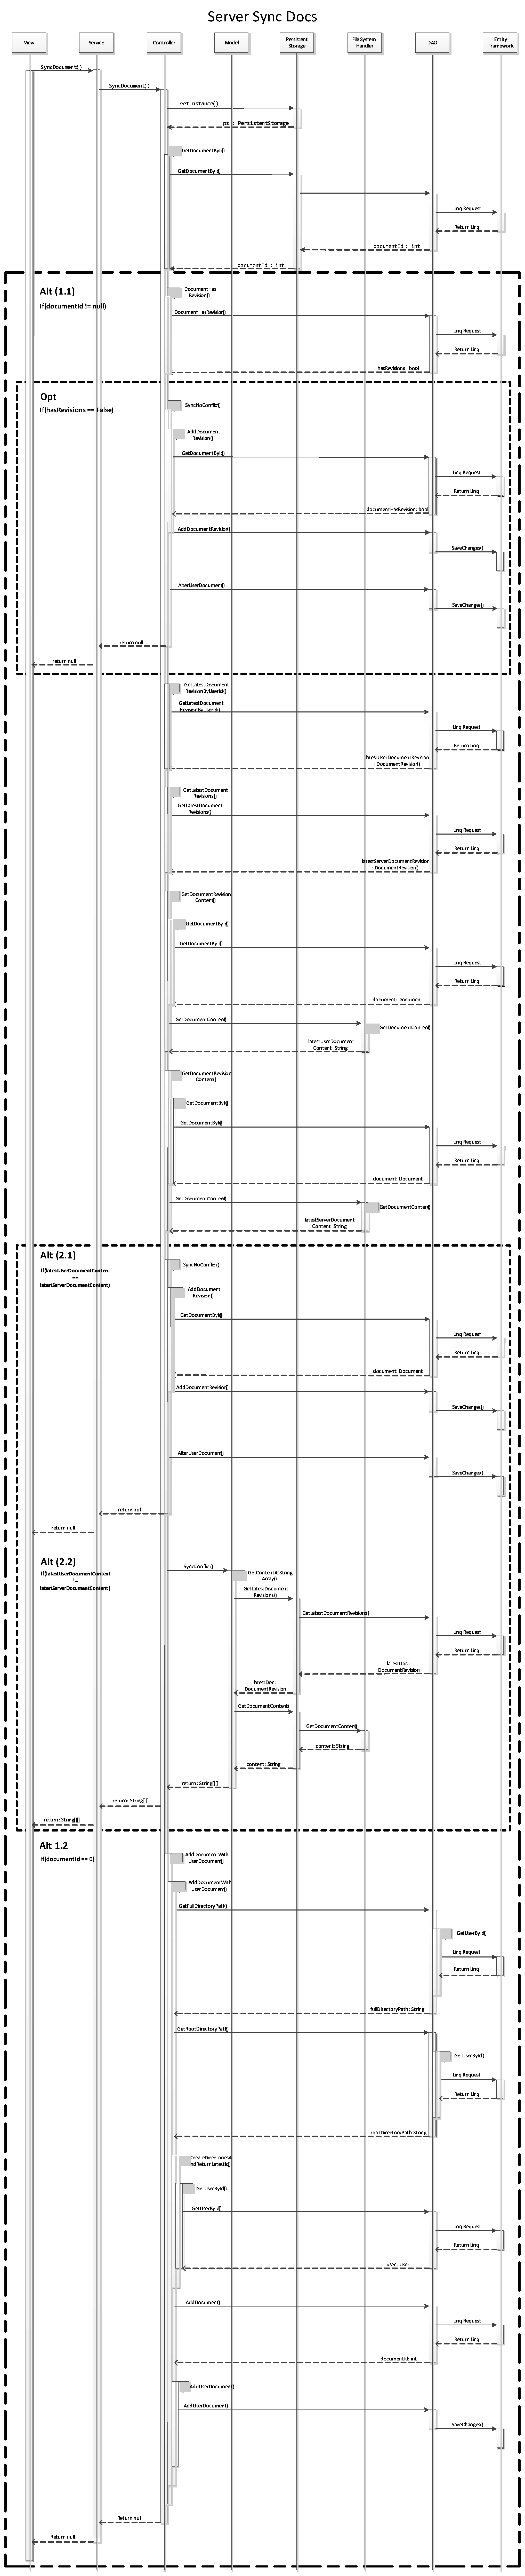
\includegraphics[width=\textwidth]{InteractionDiagramSyncDocNew.eps}
%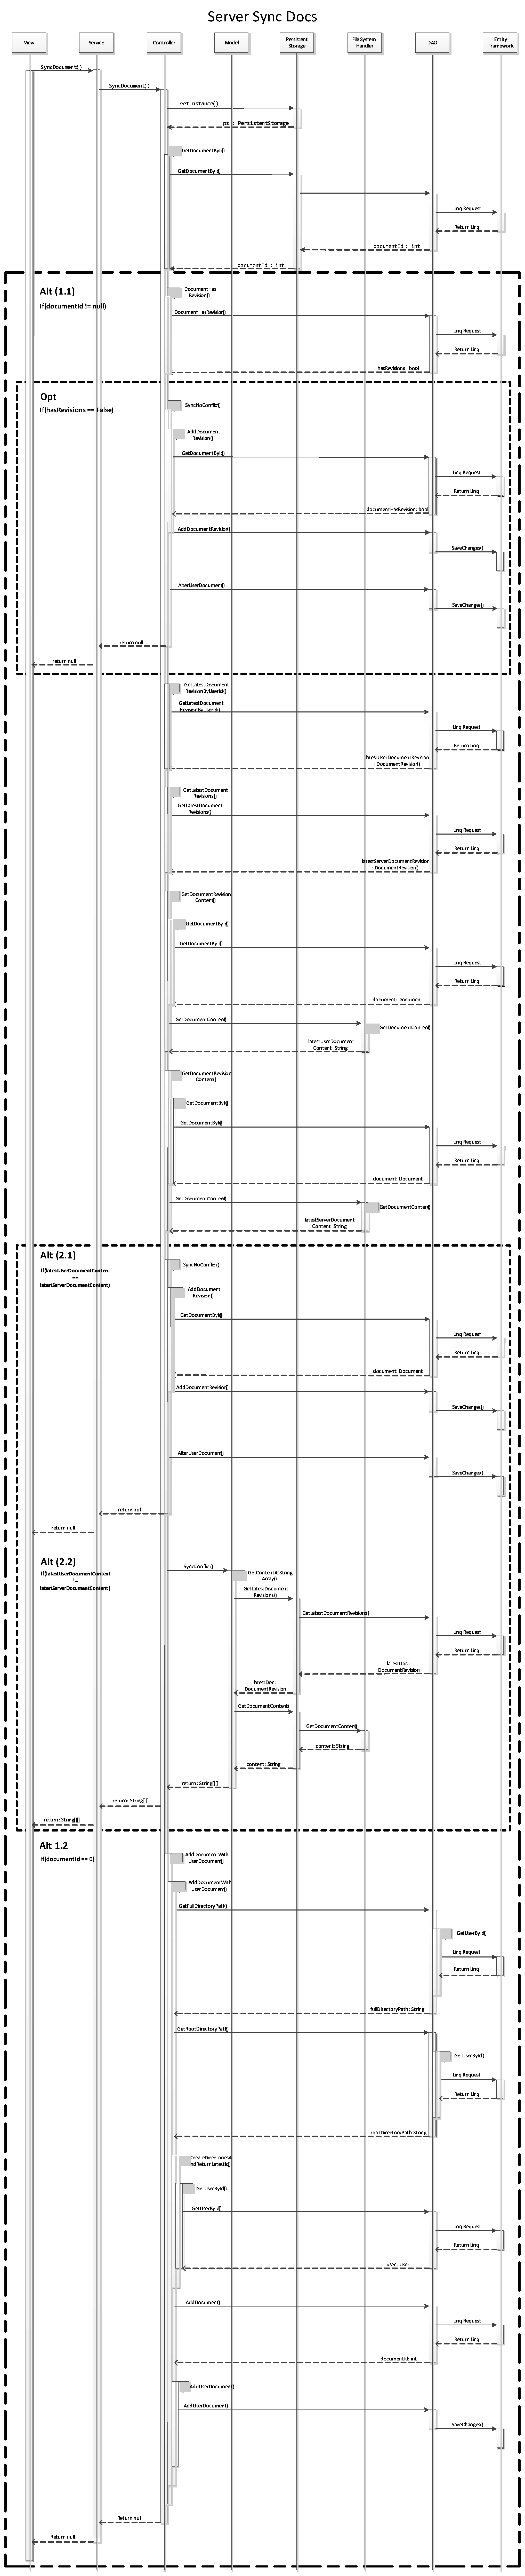
\epsfig{file=InteractionDiagramSyncDocNew.eps, width=0.9\linewidth,clip=}




\end{document}